\section{Denavit-Hartenberg}

\vspace*{-15pt}
\begin{figure}[H]
	\hspace*{10pt}
	\begin{subfigure}{0.23\columnwidth}
		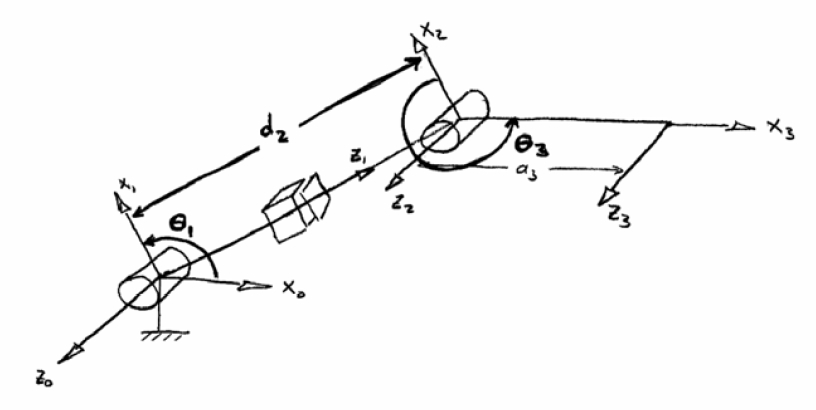
\includegraphics[align=c,angle=90,origin=c,width=\linewidth]{images/dh2}
	\end{subfigure}
%	\hspace*{pt}
	\begin{subfigure}{\columnwidth}
		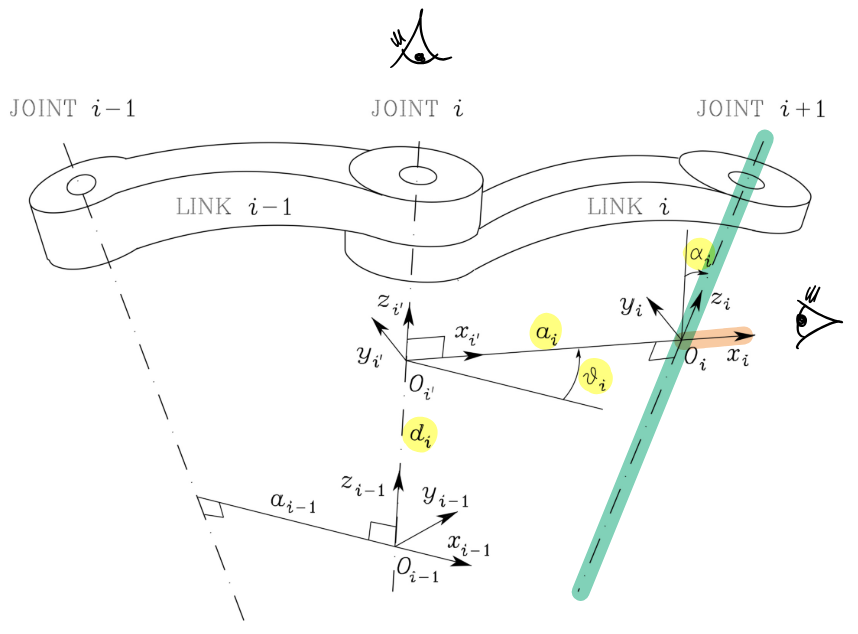
\includegraphics[align=c,width=0.7\linewidth]{images/dh}
	\end{subfigure}
\end{figure}
%\begin{figure}[H]
%	\centering
%	\includegraphics[width=0.6\linewidth]{images/kinematics_9}
%\end{figure}

Il sistema di riferimento $\mathcal{R}_i$ solidale con $\textit{LINK}_i$ viene definito secondo le seguenti regole:\\

\circled{1} \textbf{Asse $z_i$ e origine $O_i$}
\begin{itemize}
	\item \colorbox{Green}{\textbf{L’asse} $\boldsymbol{z_i}$} è posto lungo l’asse di movimento di $g_{i+1}$ (asse di rotazione o di traslazione a seconda del tipo di giunto)
	\item \textbf{L’origine} $\boldsymbol{O_i}$ è posta all’intersezione di $z_i$ con la normale comune (\textit{common normal}) fra gli assi $z_{i-1}$ e $z_i$.
	La normale comune è quella retta perpendicolare ad entrambi gli assi (nota: entrambi angoli retti nella figura)
	\item \textbf{Casi particolari}:
	\vspace*{-3pt}
	\begin{itemize}
		\item $\boldsymbol{\mathcal{R}_0}$: origine $O_0$ e $x_0$ possono essere fissati a piacimento (solo $z_0$ univocamente definito).
%		qua è univocamente definita solo la direzione di $z_0$, data dall’asse di movimento di $g_1$; l’origine $O_0$ e $x_0$ possono essere fissati a piacimento
		\item $\boldsymbol{\mathcal{R}_n}$: $\nexists \ g_{n+1} \implies z_n, \ O_n$ non univocamente definiti. Per consuetudine: origine nel centro della pinza e $z_n$ coincidente a a $z_{n-1}$ (visto che tipicamente l'ultimo giunto è rotoidale).
	\end{itemize}
\end{itemize}
\vspace*{5pt}

\circled{2} \textbf{Asse $x_i$ e $y_i$}
\begin{itemize}
	\item \colorbox{YellowOrange}{\textbf{L’asse $\boldsymbol{x_i}$}} è fissato lungo la normale comune fra gli assi $z_{i-1}$ e $z_i$
	\begin{itemize}
		\item Se $z_{i-1}$ e $z_i$ si intersecano $\implies$ direzione di $x_i$ ($\perp z_i$) è arbitraria
		%l’origine di $\mathcal{R}_i$ coincide con il loro punto di intersezione e la direzione di $x_i$ (ortogonale a $z_i$) è arbitraria
		\item se $z_{i-1}$ e $z_i$ sono paralleli $\implies$ origine arbitraria, $x_i$ nel piano normale a $z_{i-1}$ e $z_i$ con direzione e verso arbitrari.
	\end{itemize}
	\item \textbf{L’asse $\boldsymbol{y_i}$} completa la terna destrorsa ($j = k\times i$)
\end{itemize}
\vspace*{5pt}

\circled{3} \textbf{Sistema di riferimento intermedio}\\[5pt]
$z_{i'}$ diretto lungo $z_{i-1}$ $|$ $O_{i'}$ posta all’intersezione di $z_{i-1}$ con la normale comune fra $z_{i-1}$ e $z_i$ $|$ $x_{i'}$ diretto lungo la normale comune fra $z_{i-1}$ e $z_i$ (come $x_i$)

\vspace*{10pt}

\setlength{\fboxsep}{7pt} % Adjust the padding as needed
\fbox{
\begin{minipage}{0.93\columnwidth}
	\begin{itemize}
		\item $\boldsymbol{d_i} \rightarrow$ \textbf{link offset}: coordinata di $O_{i'}$ lungo $z_{i-1}$
		\item $\boldsymbol{\theta_i} \rightarrow$ \textbf{joint angle}: angolo di rotazione da $x_{i-1}$ a $x_i$ attorno all'asse $z_{i'}$ (positivo quando la rotazione è anti-oraria)
		\item $\boldsymbol{a_i} \rightarrow$ \textbf{link length}: distanza (con segno) fra $O_i$ e $O_{i'}$
		\item $\boldsymbol{\alpha_i} \rightarrow$ \textbf{link twist}: angolo di rotazione da $z_{i-1}$ a $z_i$ attorno all'asse $x_i$ (positivo quando la rotazione è anti-oraria)
	\end{itemize}

$$
{}^{i-1}\mathbf{T}_{i}(q_i)
=
\begin{bmatrix}
	c\theta_i & -s\theta_ic\alpha_i & s\theta_is\alpha_i & a_ic\theta_i \\
	s\theta_i & c\theta_ic\alpha_i & -c\theta_is\alpha_i & a_is\theta_i \\
	0 & s\alpha_i & c\alpha_i & d_i \\
	0 & 0 & 0 & 1
\end{bmatrix}
$$
\end{minipage}
}

\vspace*{7pt}
\textbf{Trigonometric inequalities}:
$$
c_{12} + s_{12} = c_{1-2}
\qquad
c_{12} - s_{12} = c_{1+2}
\qquad
s_1c_2 - c_1s_2 = s_{1-2}
\qquad
s_1c_2 + c_1s_2 = s_{1+2}
$$

\vspace*{10pt}
\textbf{Tips}:
\begin{align*}
a_i &\rightarrow
\begin{cases}
\ z_{i-1} \overset{\text{dist.}}{\longleftrightarrow} z_i \quad \text{along } x_i
\end{cases}\\
%
\alpha_i &\rightarrow
\begin{cases}
\ z_{i-1} \overset{\angle}{\longrightarrow} z_i \quad \text{around } x_i
\end{cases}\\
%
d_i &\rightarrow
\begin{cases}
\ x_{i-1} \overset{\text{dist.}}{\longleftrightarrow} x_i \quad \text{along } z_{i-1}
\end{cases}\\
%
\theta_i &\rightarrow
\begin{cases}
\ x_{i-1} \overset{\angle}{\longrightarrow} x_i \quad \text{around } z_{i-1}
\end{cases}
\end{align*}
\vspace*{-15pt}
